\section{Switch}
A network switch is a computer networking device that links network segments or network devices. The term commonly refers to a multi-port network bridge that processes and routes data at the data link layer (layer 2) of the OSI model. Switches receives a message from any device connected to it and then transmits the message only to the device for which the message was meant. This makes the switch a more intelligent device than a hub (which receives a message and then transmits it to all the other devices on its network). 
Switches may operate at one or more layers of the OSI model, including data link and network. A device that operates simultaneously at more than one of these layers is known as a multilayer switch.
\begin{figure}[htbp]
\begin{center}
	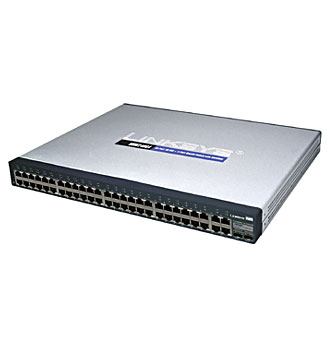
\includegraphics[width=5cm]{./Networking/ntwhardware/switch.jpg}
\caption{Switch}
\label{default}
\end{center}
\end{figure}
